\section{$z$-transform}
\subsection{$z$-transform}
\paragraph{Definition}
\begin{itemize}
    \item The $z$-transform of a sequence $x[n]$ is:
        \[
            X(z) = \sum_{n=-\infty}^{+\infty} x[n] z^{-n}
        \]
        where $z = re^{j\omega}$ is a complex variable.

    \item Recall that, the discrete-time Fourier transform is defined as
        \[
            X(e^{j\omega}) = \sum_{n=-\infty}^{+\infty} x[n] e^{-j\omega n}
        \]
    Comparing $z$-transform and DTFT, it is clear that the discrete-time Fourier transform is a special case of $z$-transform with $r=1$. Equivalently, $\lvert z \rvert = 1$, as the \textit{unit circle} with $0 \leq \omega \leq 2\pi $ shown in \autoref{fig:z_unit_circ}.
    \begin{figure}[H]
        \centering
        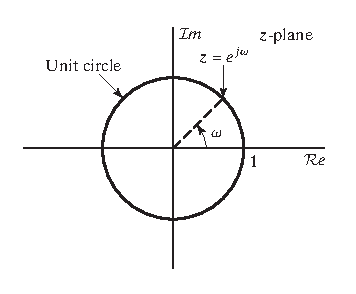
\includegraphics[width=.4\textwidth]{images/z_plane.eps}
        \caption{The unit circle with $r=1$ in the complex $z$-plane}
        \label{fig:z_unit_circ}
    \end{figure}
    This tells us that, the $z$-transform can be viewed as a generalization of the classical Fourier transform.
\end{itemize}

\paragraph{Remarks on the $z$-transform} The $z$-transform is the counterpart of the Laplace transform in the continuous time domain.
\begin{itemize}
    \item Bilateral Laplace transform:
    \[
        X(s) = \int_{-\infty}^{+\infty} x(t) e^{-st} \mathrm{d}t
    \]
    \item $z$-transform:
    \[
        X(z) = \sum_{n=-\infty}^{+\infty} x[n] z^{-n}
    \]
\end{itemize}


\subsection{Region of Convergence}

\begin{itemize}
    \item \textbf{What is the condition for DTFT to converge?} Applying the property \textit{``The magnitude of sum has to be less or equal than the sum of magnitudes"} to the magnitude of Fourier transform (DTFT):
    \begin{align*}
        \lvert X(e^{j \omega}) \rvert
        & = \bigg\lvert \sum_{n=-\infty}^{+\infty} x[n] e^{-j\omega n} \bigg\rvert \leq  \sum_{n=-\infty}^{+\infty} \lvert x[n] \rvert \lvert \cancelto{1}{e^{-j\omega n}} \rvert \\
    \end{align*}
    This conclusion helps us to determine the condition for the convergence of DTFT: if DTFT converges, $\lvert X(e^{j \omega}) \rvert < \infty$, that is
    \[
        \lvert X(e^{j \omega}) \rvert \leq \sum_{n=-\infty}^{+\infty}\lvert x[n] \rvert < \infty
    \]
    we thus only need to evaluate the value of $\sum_{n=-\infty}^{+\infty}\lvert x[n] \rvert$.

    \item \textbf{Not all Fourier transform converges!} The power series representing the Fourier transform does not converge for all sequences, the infinite sum may not always in finite.
    
    \begin{minipage}{.45\textwidth}
    \begin{ex}{}
    For $x[n] = (\frac{1}{2})^n u[n]$, the Fourier transform converges to 2:
    \[
    \sum_{n=-\infty}^{+\infty} \lvert x[n] \rvert = 2
    \]
    \end{ex}
    \end{minipage} \hfill
    \begin{minipage}{.45\textwidth}
    \begin{ex}{}
    For $x[n] = (2)^n u[n]$, the Fourier transform diverges:
    \[
    \sum_{n=-\infty}^{+\infty} \lvert x[n] \rvert = +\infty
    \]
    \end{ex}
    \end{minipage}

    \item Extending the aforementioned concept to the $z$-transform: $z$-transform does not converge for all values of $z$. For any given sequence, the region of values of $z$ for which the $z$-transform power series converges is called the \textit{region of convergence}, or \textit{ROC}.
    \[
        \lvert X(z) \rvert = \bigg\lvert  \sum_{n=-\infty}^{+\infty} x[n] z^{-n} \bigg\rvert \leq \sum_{n=-\infty}^{+\infty} \lvert x[n] \rvert \lvert z \rvert^{-n} < \infty
    \]
    we only need to evaluate the value of $\sum_{n=-\infty}^{+\infty} \lvert x[n] \rvert \lvert z \rvert^{-n}$.

    \item If the convergence condition is satisfied by an arbitrary value $z_1$, then the convergence condition is also satisfies by all values of $z$ such that $\lvert z \rvert = z_1$. Therefore, we can graphically represent the ROC for $0 \leq z_1 < \lvert z \rvert < z_2 \leq \infty$, as shown in \autoref{fig:roc}.
    
    \begin{figure}[H]
        \centering
        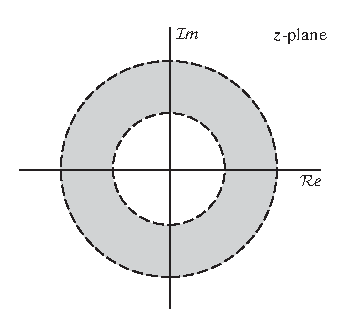
\includegraphics{images/region_of_conv.eps}
        \caption{Graphical representation of region of convergence for $0 \leq z_1 < \lvert z \rvert < z_2 \leq \infty$}
        \label{fig:roc}
    \end{figure}
\end{itemize}

\begin{ex}{ \ Sum of two exponential sequences}
    Consider a signal that is the sum of two real exponentials:
    \[
    x[n] = \bigg( \frac{1}{2} \bigg)^{n} u[n] + \bigg( -\frac{1}{3} \bigg)^{n} u[n]
    \]
    The $z$-transform is 
    \begin{align*}
        X(z) 
        & = \sum_{n=-\infty}^{+\infty} \bigg\{ \bigg( \frac{1}{2} \bigg)^{n} u[n] + \bigg( -\frac{1}{3} \bigg)^{n} u[n] \bigg\} z^{-n} \\
        & = \sum_{n=-\infty}^{+\infty} \bigg( \frac{1}{2} \bigg)^{n} u[n] z^{-n} +  \sum_{n=-\infty}^{+\infty}\bigg( -\frac{1}{3} \bigg)^{n} u[n] z^{-n} \\
        & = \sum_{n=0}^{+\infty} \bigg( \frac{1}{2} z^{-1} \bigg)^{n} +  \sum_{n=0}^{+\infty} \bigg( -\frac{1}{3} z^{-1} \bigg)^{n} \\
        & = \frac{1}{1-\frac{1}{2}z^{-1}} + \frac{1}{1+\frac{1}{3}z^{-1}} = \frac{2(1-\frac{1}{12}z^{-1})}{(1-\frac{1}{2}z^{-1})(1+\frac{1}{3}z^{-1})} \\
        & = \boxed{\frac{2z(z-\frac{1}{12})}{(z-\frac{1}{2})(z+\frac{1}{3})}}
    \end{align*}
    Poles: $z=\frac{1}{2}$, $z=-\frac{1}{3}$, zero: $z=\frac{1}{12}$. For convergence of $X(z)$, it requires both $\displaystyle \bigg\lvert (\frac{1}{2})z^{-1}\bigg\rvert < 1$ and $\displaystyle \bigg\lvert (-\frac{1}{3})z^{-1}\bigg\rvert < 1$. Equivalently, $\lvert z \rvert >\frac{1}{2}$ and $\lvert z \rvert >\frac{1}{3}$. The corresponding pole-zero plot and ROC is shown in \autoref{fig:ex3-3}.
    \begin{figure}[H]
        \centering
        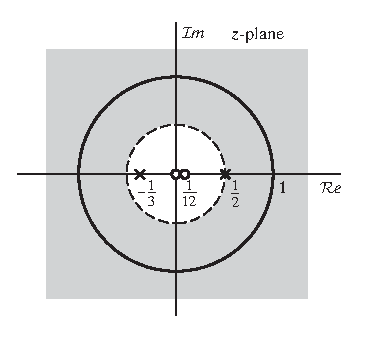
\includegraphics{images/example3-3.eps}
        \caption{Pole-zero plot and ROC for $\frac{2z(z-\frac{1}{12})}{(z-\frac{1}{2})(z+\frac{1}{3})}$}
        \label{fig:ex3-3}
    \end{figure}

    \paragraph{Remarks}
    \begin{itemize}
        \item[-] Sum of geometric sequence: $\displaystyle S_{n} = \frac{a_{1}(r_n - 1)}{r-1}$, where $a_1$ is the first term of the sequence, $r$ is the common ratio. This explains how we get the sum of exponentials above.

        \item[-] One good way to understand the convergence criterion of $X(z)$, we can think the denominator should be negative (\textit{analogous to the stability criterion for a system from Year-2 Control module}).  
    \end{itemize}
\end{ex}

\begin{ex}{ \ Finite-length truncated exponential sequence}
    Consider the signal 
    \[
    x[n] = 
    \begin{cases}
        a^n,    & 0 \leq n \leq N-1, \\
        0,      & \text{otherwise}.
    \end{cases}
    \]
    The $z$-transform is 
    \[
    X(z) = \sum_{n=0}^{N-1} a^{n}z^{-n} = \sum_{n=0}^{N-1} (az^{-1})^n = \frac{1-(az^{-1})^N}{1-az^{-1}} = \boxed{\frac{1}{z^{N-1}} \frac{z^N - a^N}{z-a}}
    \]
    The ROC is determined by the set of $z$ values for which
    \[
    \sum_{n=0}^{N-1} \lvert az^{-1} \rvert^{n} < \infty
    \]
    The sum is finite as long as $az^{-1}$ is finite, which in turn requires only $\lvert a \rvert < \infty$ and $z \neq 0$, leading to the ROC spanning over the entire $z$-plane with an exception of the origin ($z=0$). \\

    For example, with $N=16$ and $0<a<1$, the pole-zero plot is shown in \autoref{fig:ex3-6}.
    \begin{figure}[H]
        \centering
        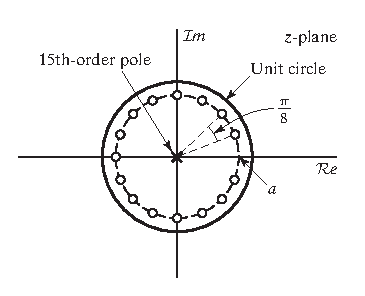
\includegraphics{images/example3-6.eps}
        \caption{Pole-zero plot with $N=16$}
        \label{fig:ex3-6}
    \end{figure}
    Specifically, the $N$ roots of the numerator polynomial are at the $z$-plane locations
    \[
    z_{k} = ae^{j(2\pi k/N)}, \quad k=0, 1, ..., N-1
    \]
\end{ex}

\subsection{Common $z$-Transform Pairs}
\begin{table}[H]
    \centering
    \begin{tabular}{c c c}
    \toprule
    \textbf{Sequence}    & \textbf{Transform}     & \textbf{ROC} \\ 
    \midrule
        $\delta[n]$     &   1   & all $z$  \\[.5em]
        
        $u[n]$     &   $\frac{1}{1-z^{-1}}$   & $\lvert z \rvert >1$  \\[.5em]
        
        $-u[-n-1]$     &   $\frac{1}{1-z^{-1}}$   &  $\lvert z \rvert <1$  \\[.5em]
        
        $\delta[n-m]$     &   $z^{-m}$   & all $z$ except 0 (if $m>0$) or $\infty$ (if $m<0$) \\[.5em]
        
        $a^{n}u[n]$     &  $\frac{1}{1-az^{-1}}$    & $\lvert z \rvert > \lvert a \rvert$\\[.5em]
        
        $-a^{n}u[-n-1]$     &  $\frac{1}{1-az^{-1}}$    & $\lvert z \rvert < \lvert a \rvert$\\[.5em]
        
        $na^{n}u[n]$     &  $\frac{az^{-1}}{(1-az^{-1})^2}$    & $\lvert z \rvert > \lvert a \rvert$\\[.5em]
        
        $-na^{n}u[-n-1]$     &  $\frac{az^{-1}}{(1-az^{-1})^2}$    & $\lvert z \rvert < \lvert a \rvert$\\[.5em]
        
        $\cos(\omega_0 n)u[n]$     &  $\frac{1-\cos(\omega_0)z^{-1}}{1-2\cos(\omega_0)\^{-1}+z^{-2}}$    & $\lvert z \rvert > 1$\\[.5em]

        $\sin(\omega_0 n)u[n]$     &  $\frac{\sin(\omega_0)z^{-1}}{1-2\cos(\omega_0)\^{-1}+z^{-2}}$    & $\lvert z \rvert > 1$\\[.5em]

        $x[n] = 
    \begin{cases}
        a^n,    & 0 \leq n \leq N-1, \\
        0,      & \text{otherwise}.
    \end{cases}$    & $\frac{1-(az^{-1})^N}{1-az^{-1}}$     & $\lvert z \rvert > 0$ \\

    \bottomrule
    \end{tabular}
\end{table}

\subsection{Properties of the $z$-transform}
For the following properties, assume
\[
    x[n] \ \xleftrightarrow[]{\mathcal{Z}} \ X(z)  \quad \quad   ROC = R_x
\]
\[
    x_1[n] \ \xleftrightarrow[]{\mathcal{Z}} \ X_1(z)  \quad \quad   ROC = R_{x1}
\]
\[
    x_2[n] \ \xleftrightarrow[]{\mathcal{Z}} \ X_2(z)  \quad \quad   ROC = R_{x2}
\]
\begin{table}[H]
    \centering
    \begin{tabularx}{\textwidth}{X c c}
    \toprule
    \textbf{Property}    & \textbf{Transform}     & \textbf{ROC} \\ 
    \midrule
        Linearity     &   $ax_1[n]+nx_2[n] \ \xleftrightarrow[]{\mathcal{Z}} \ aX_1(z)+bX_2(z)$   & all $R_{x1} \cap R_{x2}$  \\[.5em]
        
        Time shifting     &   $x[n-n_0] \ \xleftrightarrow[]{\mathcal{Z}} \ z^{-n_0} X(z)$   & $R_{x} (\text{except at $z=0$ and $z=\infty$})$  \\[.5em]
        
        Multiplication by an exponential sequence     &   $z_{0}^{n} x[n] \ \xleftrightarrow[]{\mathcal{Z}} \ X(z/z_0)$   &  $z_0R_x (\lvert z_0 \rvert \lvert z_1 \rvert < \lvert z \rvert < \lvert z_0 \rvert \lvert z_2 \rvert)$  \\[.5em]
        
        Differentiation     &   $nx[n] \ \xleftrightarrow[]{\mathcal{Z}} \ -z \frac{dX(z)}{dz}$   & $R_{x}$ \\[.5em]
        
        Conjugation     &  $ x^{*}[n] \ \xleftrightarrow[]{\mathcal{Z}} \ X^{*}(z^{*})$    & $R_{x}$\\[.5em]
        
        Time reversal    &  $x^{*}[-n] \ \xleftrightarrow[]{\mathcal{Z}} \ X^{*}(1/z^{*})$    & $\frac{1}{R_x} (1/\lvert z_2 \rvert < \lvert z \rvert < 1/\lvert z_1 \rvert)$\\[.5em]

        Convolution    &  $x_1[n] * x_2[n] \ \xleftrightarrow[]{\mathcal{Z}} \ X_{1}(z) X_{2}(z)$    & $R_{x1} \cap R_{x2}$\\[.5em]
        
    \bottomrule
    \end{tabularx}
\end{table}


\begin{ex}{}
Given that 
\[
    x_1[n] = \delta[n] + 2\delta[n-1] + \delta[n-2]
\]
\[
    x_2[n] = \delta[n] -\delta[n-1]
\]
The $z$-transforms of these two sequences are
\[
    X_1(z) = 1 + 2z^{-1} +z^{-2}
\]
\[
    X_2(z) = 1 - z^{-1}
\]
Therefore, if $y[n] = x_{1}[n] * x_{2}[n]$, then
\[
    Y(z) = X_{1}(z)X_{2}(z) = (1 + 2z^{-1} +z^{-2})(1 - z^{-1}) = 1 + z^{-1} - z^{-2} - z^{-3}
\]
\[\Updownarrow\mathcal{Z}^{-1}\]
\[
    y[n] = \delta[n] + \delta[n-1] - \delta[n-2] - \delta[n-3]
\]
\end{ex}


\subsection{LTI Systems and $z$-Transform}
\begin{itemize}
    \item An LTI system is fully characterised by its impulse response. The output $y[n]$ obtained from the input $x[n]$ is:
    \[
    y[n] = x[n] * h[n]
    \]

    \item From the convolution property of the $z$-transform
    \[
    Y(z) = H(z)X(z) 
    \]
    where $H(z) := \mathcal{Z}\{h[n]\}$ is known as the \textbf{system function} of an LTI system.
\end{itemize}

\subsection{Example Questions}
%==============================================%
\begin{q}{}
The $z$-transform of the discrete-time signal $x[n]$ converges for $\lvert a \rvert \leq \lvert z \rvert \leq \lvert b \rvert$, with $0 < \lvert a \rvert \leq \lvert b \rvert$. Which of the following statements is always correct?

\begin{enumerate}[label=(\alph*)]
    \item The discrete-time Fourier transform of $x[n]$ does not converge
    \item The discrete-time Fourier transform of $x[n]$ converges
    \item The discrete-time Fourier transform of $x[n]$ converges if $1 < \lvert a \rvert < \lvert b \rvert$
    \item The discrete-time Fourier transform of $x[n]$ converges if $\lvert a \rvert \leq 1$ and $\lvert b \rvert \geq 1$
    \item The discrete-time Fourier transform of $x[n]$ converges if $\lvert a \rvert < \lvert b \rvert < 1$
\end{enumerate}
\end{q}
%==============================================%
\begin{q}{}
Consider a linear, time-invariant (LTI) system defined by the following difference equation:
\[
    y[n] + \alpha y[n-1] = x[n]
\]
where $\alpha$ is a real number. Which of the following statements is correct?

\begin{enumerate}[label=(\alph*)]
    \item The system is casual and stable for all values of $\alpha$
    \item The system does not have poles for all values of $\alpha$
    \item The system is not causal
    \item The system has a pole for $z=-\alpha$
    \item The system has a pole for $z=\alpha$
\end{enumerate}
\end{q}
%==============================================%
\begin{q}{}
Consider the discrete-time signals $x[n] = a^{-n}u[n-1]$ (where $u[n]$ is the unit step signal and $a$ is a real and positive number different from zero). Which of the following expressions for the $z$-transform of $x[n]$ and its region of convergence (ROC) is correct?

\begin{enumerate}[label=(\alph*)]
    \item $X(z) = \frac{1}{az-1}$ with ROC $\lvert z \rvert > \frac{1}{a}$
    \item $X(z) = \frac{1}{z-a}$ with ROC $\lvert z \rvert > a$
    \item $X(z) = \frac{1}{z+a}$ with ROC $\lvert z \rvert < \frac{1}{a}$
    \item $X(z) = \frac{1}{az-1}$ with ROC $\lvert z \rvert < \frac{1}{a}$
    \item $X(z) = \frac{1}{z-a}$ with ROC $\lvert z \rvert < a$
\end{enumerate}
\begin{flushright}
\begin{blueenv}
    ANS: (a)
\end{blueenv}
\end{flushright}
\end{q}
%==============================================%
\begin{q}{}
Consider the LTI system with the following impulse response $h[n]=\delta[n]-2\delta[n-\dfrac{k}{2}]+\delta[n-k]$, with $k$ an even number.
\begin{enumerate}[label=(\alph*)]
    \item Is the system stable? Is it causal? 
    \begin{flushright}
    \begin{blueenv}
        ANS: stable and casual.
    \end{blueenv}
    \end{flushright}
    
    \item Determine the system function and the transfer function, as a function of $k$.
    \begin{flushright}
    \begin{blueenv}
        ANS: $H(z) = ( 1 - e^{-j\omega \frac{k}{2}} )^2$.
    \end{blueenv}
    \end{flushright}
    
    \item Determine the phase and the group delay of the system, as a function of $k$.
    \begin{flushright}
    \begin{blueenv}
        ANS: $\angle H(e^{j\omega}) = -\frac{k}{2} \omega - \pi$, delayed by $k/2$.
    \end{blueenv}
    \end{flushright}
\end{enumerate}
    
    % {\color{blue}
    % \paragraph{Answer (a)}
    % The system is stable since it has a finite length impulse. The system is causal since for $n<0$, $h[n] = 0$.
    
    % \paragraph{Answer (b)}
    % Compute the $z$-transform of the signal
    % \begin{align*}
    %     h[n] \ & \xleftrightarrow[]{\mathcal{Z}} \ H(z) = 1 - 2z^{-\frac{k}{2}} + z^{-k} \\
    %     & \Rightarrow \ H(e^{j\omega}) = 1 - 2e^{-j\omega \frac{k}{2}} + e^{-j\omega k} = ( 1 - e^{-j\omega \frac{k}{2}} )^2 
    % \end{align*}
    % \color{blue}
    % \paragraph{Answer (c)}
    % From (b), the system function can be re-arranged as
    % \begin{align*}
    %     H(e^{j\omega}) 
    %     &= [e^{-j\omega\frac{k}{4}} (e^{j\omega\frac{k}{4}} - e^{-j\omega\frac{k}{4}})]^2 \\
    %     & = e^{-j\omega\frac{k}{2}} \left[2j\sin \left(\frac{k}{4}\omega \right) \right]^2 \\
    %     & = -4e^{-j\omega\frac{k}{2}} \sin^2 \left(\frac{k}{4}\omega\right) \\
    %     & = +4e^{-j\omega\frac{k}{2}}e^{-j\pi} \sin^2 \left(\frac{k}{4}\omega\right)
    % \end{align*}
    % Hence, the phase of the system is
    % \[
    %     \angle H(e^{j\omega}) = -\frac{k}{2} \omega - \pi,
    % \]
    % with the group delay at $k/2$.
    % }
\end{q}




